\section{Introduction}
\label{sec:intro}

Frozen flow-matching Vision-Language-Action (VLA) models offer a compelling deployment paradigm: a single pretrained policy can handle diverse manipulation tasks without retraining~\cite{black2024pi0,shukor2025smolvla,lipman2023flow}. Yet their action quality is bounded by the pretrained weights, and fine-tuning remains expensive when new tasks arrive frequently. Post-hoc learned correction, a lightweight module that refines actions at inference time without modifying VLA weights~\cite{snell2024scaling}, is an appealing alternative. But does it actually help?

\begin{figure}[t]
  \centering
  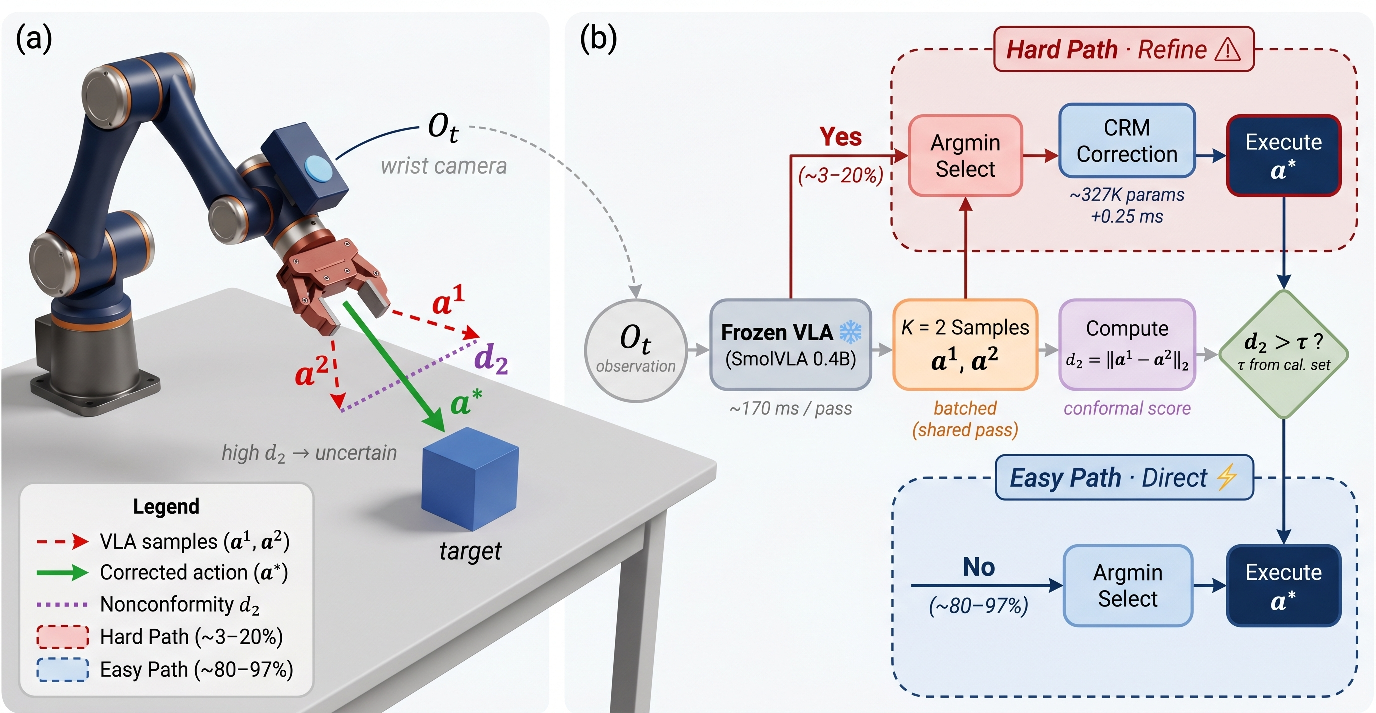
\includegraphics[width=\linewidth, trim=2 0 7 11, clip]{fig1_pipeline.pdf}
  \caption{Calibrated gating pipeline. $K{=}2$ action samples are drawn from the frozen VLA; their pairwise $L_2$ distance forms a calibrated uncertainty score. When the score falls below $\tau$ (confident step), the argmin-to-centroid sample is output directly. When it exceeds $\tau$ (uncertain step), a lightweight Correction Residual Module (CRM) applies bounded correction ($\|\boldsymbol{\delta}\|_2 \leq \varepsilon$).}
  \label{fig:pipeline}
\end{figure}

We systematically evaluate this idea and find a surprising negative result: unconditional learned correction is consistently harmful across all evaluated configurations. Across four LIBERO manipulation suites~\cite{liu2023libero} and two VLAs spanning nearly an order of magnitude in scale (0.4B to 3.6B), applying a correction module at every control step consistently degrades performance (Section~\ref{sec:failure_modes}). The problem is not the correction module itself, but the assumption that every step needs correction.

Prior work either corrects unconditionally~\cite{a2c2_2025}, quantifies uncertainty without learned correction~\cite{chen2026reconvla}, or requires RL~\cite{liu2026scvla} or slow evolutionary search ($2.41$\,s/step)~\cite{li2025vlapilot}. None analyze when correction helps versus hurts, nor provide a mechanism to suppress it on confident steps.

Our analysis reveals the root cause: on the four evaluated suites, 80--97\% of control steps already produce confident, near-deterministic actions; corrections on these steps inject noise rather than signal. The direct consequence is that knowing \emph{when not to correct} matters more than the correction's magnitude---the correction module is effective, but only on the 3--20\% of steps where the VLA is genuinely uncertain. We propose a simple gating mechanism: two stochastic action samples drawn in a single batched forward pass provide a per-step uncertainty estimate at zero extra latency. A calibrated threshold on their pairwise distance gates correction to the small fraction of genuinely uncertain steps, while the VLA's own output passes through on confident steps. This selective prediction approach~\cite{chow1970optimum,geifman2017selective} restricts correction to the minority of steps where it is most needed.

On SmolVLA~\cite{shukor2025smolvla} (0.4B) across four LIBERO suites, selective gating recovers nearly all degradation from unconditional correction. Cross-VLA experiments on $\pi_{0.5}$~\cite{black2025pi05} (3.6B) with $n{=}3$ seeds per condition confirm that the failure pattern persists and amplifies on stronger models. Threshold sensitivity analysis shows that gating is robust to $\tau$ choice, and trigger rate shows a positive trend with net improvement over VLA-only across suites (Appendix~\ref{sec:tau_sweep}).

Our contributions are:
\begin{enumerate}[leftmargin=*,nosep]
  \item \textbf{Failure analysis of unconditional correction} (Section~\ref{sec:failure_modes}): we show that applying learned correction at every step degrades frozen VLAs across all evaluated task suites and model scales, and identify confident steps (where the VLA needs no help) as the source of harm.
  \item \textbf{Calibrated gating via pairwise uncertainty} (Section~\ref{sec:method}): two action samples yield a per-step uncertainty proxy that gates correction to the small fraction of uncertain steps, recovering nearly all degradation on SmolVLA at zero extra latency.
  \item \textbf{Cross-VLA validation and deployment guidelines} (Section~\ref{sec:experiments}; Appendix~\ref{sec:cross_vla}): the degradation pattern generalizes from SmolVLA (0.4B) to $\pi_{0.5}$ (3.6B) with $n{=}3$ seeds per condition, and five data-grounded deployment rules---including trigger rate as a zero-cost diagnostic---enable practitioners to predict whether correction will help for a given task distribution without full evaluation.
\end{enumerate}
